\documentclass[20pt]{report}
\usepackage{inputenc,fancyhdr,listings}
\usepackage{fontspec,amsfonts,amsmath,amssymb}
\usepackage{geometry,multicol,hyperref,graphicx}
\usepackage{lipsum,pgfplots,tikz}

\geometry{a4paper, left=2.5cm, right=2.5cm, top=2.5cm, bottom=2.5cm}

\title{\huge \textbf{MANSI - Mathematical and Statistical Interface}}

\author{\Large Mandar Sharad Bhosale}
\date{\today}
\pagestyle{fancy}

\fancyfoot[R]{\thepage}
\fancyfoot[L]{\thesection}
\fancyfoot[C]{\rightmark}

\renewcommand{\headrulewidth}{0.4pt}
\renewcommand{\footrulewidth}{0.4pt}
\begin{document}
\maketitle
\tableofcontents

\listoffigures
\listoftables
\begin{abstract}
   MANSI, a comprehensive educational platform for mathematics and statistics, addresses the challenges of traditional teaching methods and lack of personalized support through a user-centered design, adaptive learning technology, and engaging interactive experiences. The platform's development involved defining requirements, designing architecture, creating content, testing and refining, and deploying and maintaining the system. MANSI's key features include personalized learning paths, adaptive learning, personalized feedback, collaborative learning environment, and comprehensive content coverage. With its emphasis on personalization, adaptability, and engagement, MANSI revolutionizes mathematics and statistics education, catering to diverse learners and enhancing their understanding and retention of these crucial subjects.
\end{abstract}
\chapter{Preliminary}
Mathematics and statistics are foundational disciplines that play a crucial role in understanding and interpreting the world around us. Whether you're interested in scientific research, business analytics, data science, or simply enhancing your problem-solving skills, a strong foundation in mathematics and statistics is essential.
\paragraph{Mathematics:}Mathematics is the language of patterns, relationships, and structures. It provides a framework for logical reasoning and problem-solving. Studying mathematics involves exploring concepts such as algebra, calculus, geometry, and discrete mathematics. These topics not only sharpen analytical thinking but also have wide-ranging applications in fields like physics, engineering, economics, and computer science.

\paragraph{Statistics:}Statistics, on the other hand, is the science of collecting, analyzing, interpreting, presenting, and organizing data. It involves methods for drawing conclusions from data and making informed decisions. Statistical techniques are used in diverse fields like biology, psychology, economics, and sociology to uncover patterns, test hypotheses, and extract meaningful insights from complex datasets.

\begin{figure}
    \centering
    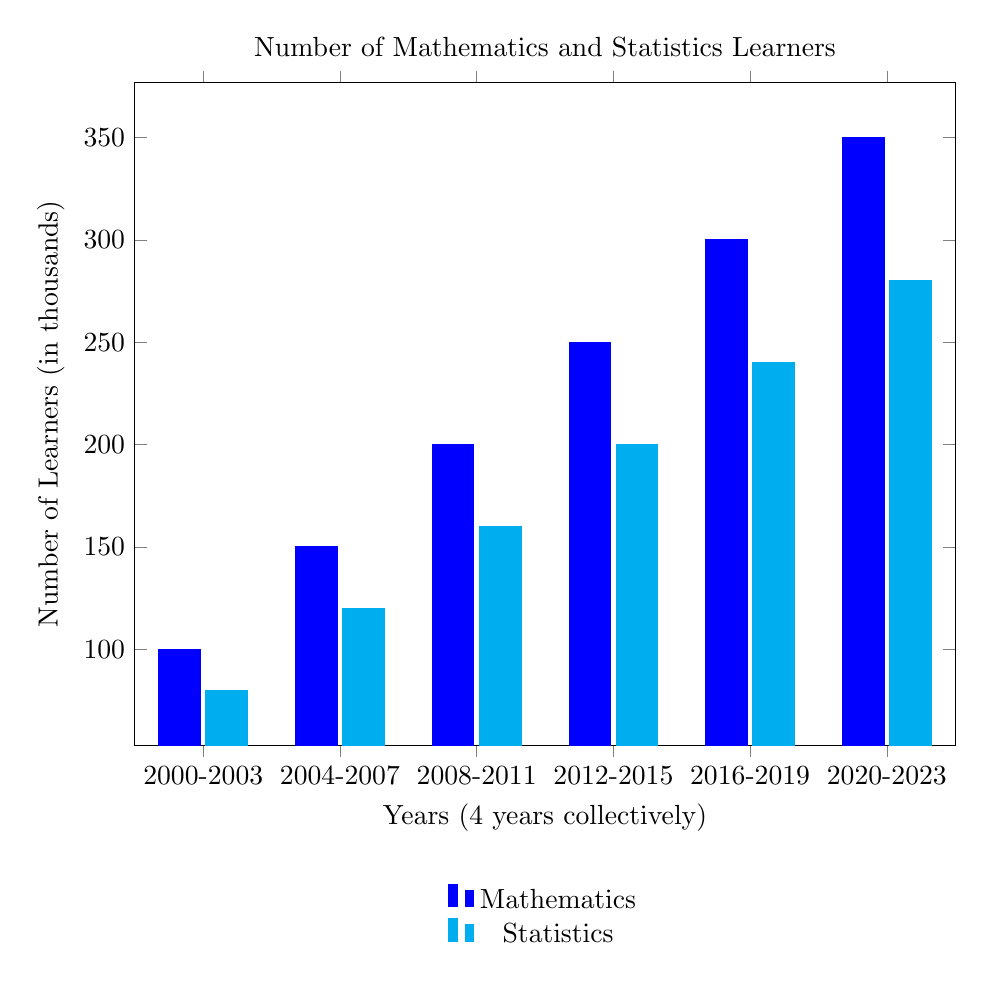
\begin{tikzpicture}
        \begin{axis}[
            width=12cm,
            height=10cm,
            title={Number of Mathematics and Statistics Learners},
            xlabel={Years (4 years collectively)},
            ylabel={Number of Learners (in thousands)},
            xtick=data,
            xticklabels={2000-2003, 2004-2007, 2008-2011, 2012-2015, 2016-2019, 2020-2023},
            legend style={at={(0.5,-0.2)},anchor=north, draw=none},
            ybar,
            bar width=15pt,
        ]
        
        % Replace the data below with actual data
        \addplot[blue,fill=blue] coordinates {(1,100) (2,150) (3,200) (4,250) (5,300) (6,350)};
        \addlegendentry{Mathematics}
        
        % Replace the data below with actual data
        \addplot[cyan,fill=cyan] coordinates {(1,80) (2,120) (3,160) (4,200) (5,240) (6,280)};
        \addlegendentry{Statistics}
        
        \end{axis}
        
    \end{tikzpicture}
    \caption{Number of Mathematics and Statistics Learners over the Years}
\end{figure}


\section{Purpose and Challenges \\ to Learn Mathematics and Statistics}
There are many aspects in learning mathematics and statistics. Most of the learners use the traditional way to learn mathematics and statistics. In this generation, learners need a platform where they can have integrated platform.
\subsection{why we learn mathematics and statistics}
Whether you're a student aiming to excel in your academic pursuits, a professional seeking to enhance your skill set, or someone with a general interest in quantitative reasoning, learning mathematics and statistics empowers you to navigate a world that increasingly relies on data and analytical thinking.

\begin{itemize}
    \item \textbf{Problem Solving:} Mathematics teaches systematic problem-solving skills, providing tools to analyze and tackle complex issues.
    \item \textbf{Data Literacy:} Statistics equips individuals with the ability to make sense of data, making informed decisions in an increasingly data-driven world.
    \item \textbf{Career Opportunities:} Proficiency in mathematics and statistics opens doors to various career paths, including data analysis, finance, research, and technology.
    \item \textbf{Scientific Inquiry:} These disciplines are fundamental to scientific research, enabling the formulation and testing of hypotheses.
\end{itemize}
\subsection{Challenges}

Despite the invaluable benefits of mathematics and statistics, many students face challenges in learning these subjects. These challenges often stem from the abstract nature of the concepts, traditional teaching methods, and a lack of personalized support.

\begin{itemize}

\item \textbf{Abstraction and Conceptual Difficulty:} Mathematics and statistics often involve abstract concepts and unfamiliar symbols, which can make it challenging for some students to grasp and understand. The lack of concrete examples and real-world applications can further hinder comprehension.

\item \textbf{Traditional Teaching Methods:} Traditional teaching methods that rely on rote memorization and passive learning can make mathematics and statistics less engaging and discouraging for students. These methods fail to cater to individual learning styles and preferences, leading to disinterest and a lack of motivation.

\item \textbf{Lack of Personalized Support and Feedback:} Students may face difficulties in finding personalized support and timely feedback, hindering their ability to identify and address their learning gaps. This lack of individualized attention can lead to frustration and a sense of being overwhelmed.
\end{itemize}

\section{The need of IT Tools in Mathematics and Statistics Education}

In today's technology-driven world, the integration of IT tools into education has become increasingly crucial. This is particularly evident in the fields of mathematics and statistics, where IT tools offer a multitude of benefits to enhance the learning process and foster deeper understanding.

\subsection{Overcoming Traditional Challenges}

Traditionally, mathematics and statistics education has faced challenges such as:

\begin{enumerate}

\item \textbf{Abstract Nature of Concepts:} Mathematical and statistical concepts are often abstract and difficult to grasp, leading to disengagement and misconceptions among students.

\item \textbf{Passive Learning Methods:} Traditional teaching methods often rely on passive learning techniques, such as rote memorization and lectures, which fail to cater to diverse learning styles and hinder active engagement.

\item \textbf{Lack of Personalized Support:} Students may face difficulties in finding individualized support and timely feedback, which can hinder their ability to identify and address their learning gaps.

\end{enumerate}

IT tools address these challenges by providing personalized learning experiences, interactive content, and adaptive feedback, making mathematics and statistics more accessible and engaging for all learners.

\subsection{Enhancing Comprehension and Retention}

IT tools provide various means to enhance students' comprehension and retention of mathematical and statistical concepts:

\begin{itemize}

\item \textbf{Visualization and Simulations:} IT tools enable the visualization of abstract concepts, allowing students to see and interact with mathematical models and statistical distributions. This visual representation aids in understanding the underlying principles and patterns.

\item \textbf{Interactive Exercises and Games:} Interactive exercises and gamification elements make learning more engaging and stimulating, motivating students to practice problem-solving and reinforce their understanding.

\item \textbf{Adaptive Learning Pathways:} IT tools can tailor the learning path to each student's individual needs and pace, providing appropriate difficulty levels and personalized feedback to maximize their learning progress.

\end{itemize}

\subsection{Developing Problem-solving Skills}

IT tools foster the development of problem-solving skills in mathematics and statistics:

\begin{itemize}

\item \textbf{Step-by-step Solutions and Explanations:} IT tools can provide step-by-step solutions to problems, explaining the reasoning behind each step and highlighting the underlying mathematical principles.

\item \textbf{Interactive Problem-solving Environments:} Interactive problem-solving environments allow students to practice solving problems in real-time, receiving immediate feedback and guidance as they progress.

\item \textbf{Real-world Applications and Data Analysis:} IT tools can integrate real-world data and applications, enabling students to apply their mathematical and statistical knowledge to practical scenarios and solve real-world problems.

\end{itemize}

\subsection{Fostering Collaboration and Communication}

IT tools promote collaboration and communication in mathematics and statistics education:

\begin{itemize}

\item \textbf{Online Discussion Forums and Collaborative Workspaces:} IT tools facilitate online discussions and collaborative workspaces, allowing students to interact with peers, share ideas, and work together on projects.

\item \textbf{Peer-to-peer Learning and Feedback:} Online platforms enable peer-to-peer learning and feedback, where students can learn from each other, share their understanding, and provide constructive feedback.

\item \textbf{Teacher-student Interactions and Personalized Guidance:} IT tools enhance teacher-student interactions, providing teachers with real-time insights into student progress and allowing for personalized guidance and support.

\end{itemize}

In conclusion, IT tools play an essential role in mathematics and statistics education by overcoming traditional challenges, enhancing comprehension and retention, developing problem-solving skills, and fostering collaboration and communication. As technology continues to evolve, the integration of IT tools will further revolutionize the teaching and learning of these crucial subjects.\\


\begin{table}
    \centering
    \begin{tabular}{|c|c|c|}
        \hline
        \textbf{Tool} & \textbf{Purpose} & \textbf{Year of Development} \\
        \hline
        \href{https://www.latex-project.org/}{\LaTeX} & Document preparation system & 1983 \\
        \hline
        \href{https://www.r-project.org/}{R} & Statistical computing and graphics & 1993 \\
        \hline
        \href{https://www.python.org/}{Python} & General-purpose programming language with math libraries & 1991 \\
        \hline
        \href{https://www.wolfram.com/mathematica/}{Mathematica} & Symbolic computation and visualization & 1988 \\
        \hline
        \href{https://www.gnu.org/software/octave/}{GNU Octave} & Numerical computing similar to MATLAB & 1994 \\
        \hline
    \end{tabular}
    \caption{IT Tools for Learning and Documenting Mathematical and Statistical Studies}
    \label{tab:it_tools}
\end{table}


\chapter{What is MANSI?}
Basically MANSI is acronym for \textbf{M}athematical \textbf{AN}d \textbf{S}tatistical \textbf{I}nterface. 
It is an interactive interface to study, understand Mathematics and Statistics.
MANSI is an educational platform for mathematics and statistics that enhances learning, research, and collaboration.
It offers a vast collection of theorems and AI-generated solved examples, as well as interactive learning modules with step-by-step explanations.
The platform has an eye-catching design and an intuitive user interface, and includes a LaTeX extension for seamless thesis and academic paper writing.
MANSI also provides collaborative learning spaces for peer interaction, virtual tutoring with personalized assistance, and a research repository for access to published papers and case studies.
Gamification elements are included for motivation, and the platform seamlessly integrates with online tools and is accessible through a mobile application.

\begin{enumerate}

\item \textbf{Latex Documentation for Making Research Papers and Notes}:- MANSI provides comprehensive Latex documentation to assist students in creating well-structured and professionally formatted research papers and notes. The documentation covers the fundamentals of Latex syntax, formatting elements, and advanced features, enabling students to produce high-quality academic documents. 
\item \textbf{Problem Solver}
MANSI's interactive problem solver provides a step-by-step approach to solving mathematics and statistics problems. Students can input their problem and MANSI will guide them through the solution process, providing detailed explanations and justifications for each step. This feature helps students develop problem solving skills, identify patterns, and overcome common mistakes.

\item \textbf{Concept Notes and Solved Examples}
MANSI offers concise and clear concept notes that summarize key mathematical and statistical concepts. These notes provide a quick overview of essential definitions, formulas, and theorems, serving as a valuable reference for students. Additionally, MANSI provides a collection of solved examples that demonstrate the application of concepts in real-world scenarios, enhancing students' understanding and ability to apply their knowledge.

\item \textbf{AI-Generated Quizzes and Tests}
MANSI utilizes AI to generate personalized quizzes and tests, adapting to each student's individual progress and performance. These assessments help students gauge their understanding of concepts, identify areas for improvement, and prepare for upcoming exams. The AI-powered approach ensures that the assessments are tailored to the student's current level of knowledge, providing a more effective learning experience.
\item \textbf{Chatbot MANDAR}:
MANSI's chatbot, MANDAR, serves as a friendly and helpful companion throughout the student's learning journey. MANDAR can answer questions, provide explanations, offer guidance, and even engage in casual conversations. This interactive feature provides students with personalized support, fostering a sense of connection and reducing the barriers to seeking assistance.
\end{enumerate}
\section{How it Will Work}

At the heart of MANSI's transformative approach lies its personalized learning methodology, which tailors the educational experience to each student's unique needs, learning style, and pace. This personalization is orchestrated by a sophisticated interplay of artificial intelligence (AI) and machine learning (ML) algorithms that continuously gather and analyze data on student progress, performance, and learning preferences.

\subsection{Initial Assessment and Profile Creation}

Upon enrolling in MANSI, students undergo an initial assessment that gauges their current knowledge level, mathematical aptitude, and learning style preferences. This assessment forms the foundation of the student's personalized learning profile, which serves as a dynamic guide for MANSI's adaptive learning system.

\subsection{Real-time Data Collection and Analysis}

Throughout their learning journey, MANSI continuously monitors student interactions, performance on assessments, completion of exercises, and engagement with content. This real-time data collection provides valuable insights into each student's strengths, weaknesses, and areas for improvement.

\subsection{AI-Powered Adaptive Learning}

MANSI's AI and ML algorithms employ sophisticated techniques to analyze the collected data, identifying patterns, correlations, and trends that reveal each student's unique learning trajectory. Based on this analysis, the system dynamically adjusts the learning path for each student, selecting appropriate content, recommending challenging exercises, and providing personalized feedback.

\subsection{Personalized Learning Path Creation}

For each student, MANSI creates a personalized learning path that aligns with their individual needs and goals. This path may include:

Tailored Content Delivery: MANSI selects and delivers content that is relevant to the student's current understanding and interests, ensuring they are not overwhelmed or underchallenged.

Adaptive Difficulty Levels: The difficulty of exercises and assessments is dynamically adjusted based on the student's performance, ensuring they are constantly engaged and challenged.

Personalized Feedback Mechanisms: MANSI provides timely and personalized feedback that is tailored to each student's errors and misconceptions, helping them identify areas for improvement and refine their understanding.

Engaging Interactive Experiences: MANSI incorporates interactive exercises, simulations, and gamification elements that cater to the student's preferred learning style, making the learning process more engaging and enjoyable.

\subsection{Continuous Improvement and Dynamic Adaptation}
MANSI's AI and ML algorithms are continuously learning and adapting, refining their ability to personalize the learning experience based on the ever-growing pool of student data. This constant improvement ensures that MANSI remains at the forefront of adaptive learning, providing each student with the most effective and personalized learning experience possible.\\
In essence, MANSI's personalized learning approach transforms the educational landscape, breaking free from the one-size-fits-all approach of traditional methods. Using AI and machine learning (ML), MANSI empowers each student to learn at their own pace, maximize their understanding, and develop a genuine love for mathematics and statistics.
\section{MANDAR: AI-Powered Assistant}

MANDAR, an acronym for "Mathematical Assistant for Numerical and Derivation with Analysis and Research," is an intelligent conversational assistant specifically designed to enhance the learning of mathematics and statistics. It utilizes a sophisticated combination of AI and ML techniques to provide personalized learning experiences, comprehensive explanations, and real-time support to students.

\subsection{MANDAR's Core Functionalities}

MANDAR's primary functionalities include:

\begin{itemize}

\item \textbf{Answering Questions:} MANDAR can answer a wide range of questions related to mathematics and statistics, from basic concepts to complex problem-solving strategies. It draws upon its vast knowledge base and AI algorithms to provide accurate and comprehensive explanations.

\item \textbf{Providing Personalized Feedback:} MANDAR analyzes students' work and provides personalized feedback, identifying areas of strength and areas for improvement. It guides students towards correcting their mistakes and refining their understanding.

\item \textbf{Generating Practice Exercises:} MANDAR can generate customized practice exercises tailored to each student's current level of knowledge and skill. This personalized approach ensures that students receive the appropriate level of challenge to reinforce their understanding.

\item \textbf{Explaining Solutions and Concepts:} MANDAR can step-by-step explain the solutions to mathematical and statistical problems, providing clear and concise explanations of the underlying concepts and reasoning.
\end{itemize}
\subsection{Integrating MANDAR within MANSI}

MANDAR seamlessly integrates within MANSI, the Mathematical Analysis and Symbolic Integration environment, offering a powerful and versatile platform for mathematical exploration and problem-solving. MANSI provides a user-friendly interface for symbolic computation, while MANDAR augments this with its ability to interact with users in natural language and provide personalized guidance. This integration enables users to:

\begin{itemize}
\item Formulate Mathematical Problems in Natural Language: Users can express their mathematical problems and queries in natural language, allowing MANDAR to understand the intent and translate it into MANSI's symbolic language.

\item Receive Step-by-step Solutions and Explanations: MANDAR can break down complex mathematical problems into manageable steps, providing detailed explanations and justifications for each step. This step-by-step approach enhances understanding and promotes self-learning.

\item Visualize Mathematical Concepts and Formulas: MANDAR can generate interactive visualizations and graphs to illustrate mathematical concepts and formulas, enhancing understanding and making abstract concepts more concrete.

\item Explore Mathematical Relationships and Patterns: MANDAR can help users explore mathematical relationships and patterns by providing insights into mathematical connections and suggesting alternative approaches.

\item Generate Practice Exercises and Personalized Feedback: MANDAR can generate personalized practice exercises tailored to each user's level of understanding and identify areas for improvement, providing timely feedback and guidance.

The seamless integration of MANDAR within MANSI creates a synergistic environment where the strengths of both tools complement each other. MANSI provides the computational power and symbolic manipulation capabilities, while MANDAR acts as a natural language interface and personalized assistant, making mathematics more accessible, engaging, and effective for users of all levels.
\end{itemize}
\section{Overview}
Mathematics and statistics play a crucial role in various fields, from science and technology to finance and social sciences. Mastering these subjects is essential for critical thinking, problem-solving, and decision-making. However, traditional teaching methods often fail to address the abstract nature of mathematical and statistical concepts, leading to disengagement and misconceptions among students.

The integration of IT tools into mathematics and statistics education offers a promising solution to these challenges. IT tools provide interactive and engaging learning experiences, personalized feedback, and adaptive learning pathways, catering to diverse learning styles and enhancing comprehension.

MANSI, a comprehensive mathematical analysis and symbolic integration environment, stands at the forefront of this revolution. By seamlessly integrating with MANDAR, an AI-powered mathematical assistant, MANSI creates a powerful and versatile platform that transforms the way students learn and interact with mathematics and statistics.

Through natural language interactions, step-by-step explanations, interactive visualizations, personalized feedback, and a rich repository of mathematical knowledge, MANSI empowers students to overcome learning barriers, develop problem-solving skills, and foster a deeper understanding of these essential subjects.
\chapter{Creating Phase}
\chapter{Post-Creation Phasw}
\chapter{MANDAR}

\section{Introduction to MANDAR}
\begin{center}
    \includegraphics[height=4cm]{AIbot.jpg}
\end{center}
In the realm of education, artificial intelligence (AI) has emerged as a transformative force, revolutionizing the way students learn and interact with educational content. One such AI-powered innovation is MANDAR, an intelligent conversational assistant specifically designed to enhance the learning of mathematics and statistics. The name of MANDAR stands for "\textbf{M}athematical \textbf{A}ssistant for \textbf{N}umericals and \textbf{D}erivation with \textbf{A}nalysis and \textbf{R}esearch" reflecting its core focus on these two crucial subjects.

\subsection{MANDAR's Role in the Learning Process}

MANDAR serves as a personalized companion for students throughout their learning journey, providing a range of assistance and support. Its primary functionalities include the following.

\begin{enumerate}

\item Answering questions: MANDAR can answer a wide range of questions related to mathematics and statistics, from basic concepts to complex problem-solving strategies. It draws upon its vast knowledge base and AI algorithms to provide accurate and comprehensive explanations.

\item Providing Personalized Feedback: MANDAR analyzes students' work and provides personalized feedback, identifying areas of strength and areas for improvement. It guides students towards correcting their mistakes and refining their understanding.

\item Generating Practice Exercises: MANDAR can generate customized practice exercises tailored to each student's current level of knowledge and skill. This personalized approach ensures that students receive the appropriate level of challenge to reinforce their understanding.

\item Explaining Solutions and Concepts: MANDAR can step-by-step explain the solutions to mathematical and statistical problems, providing clear and concise explanations of the underlying concepts and reasoning.

\end{enumerate}

\section{MANDAR's Inner Workings}

The power of MANDAR lies in its sophisticated combination of AI and ML techniques, including:
The power of MANDAR lies in its sophisticated combination of AI and ML techniques, including:
\begin{enumerate}
\item \textbf{APIs}

\begin{itemize}

\item \textbf{Mathematical Formula APIs:} MANDAR utilizes APIs such as MathJax and SymPy to access and display mathematical formulas and symbols accurately within its conversational interface.

\item \textbf{Statistical Data APIs:} MANDAR integrates with statistical data providers like Quandl and Kaggle to access real-world datasets for generating practice exercises, providing real-world applications of statistical concepts.

\item \textbf{Educational Content APIs:} MANDAR connects with educational content APIs like Khan Academy and OpenStax to access curated educational resources, such as video tutorials, interactive simulations, and practice problems.

\end{itemize}

\item \textbf{ML, AI, and GPT Models}

\begin{itemize}

\item \textbf{Natural Language Processing (NLP):} NLP techniques enable MANDAR to understand and interpret natural language input from students, extracting key information, identifying their intent, and formulating appropriate responses. NLP libraries like spaCy and NLTK play a crucial role in MANDAR's ability to comprehend student queries and provide accurate responses.

\item \textbf{Machine Learning (ML):} ML algorithms are employed to train MANDAR's conversational model, improving its ability to generate personalized responses, provide tailored feedback, and adapt to each student's unique learning style. ML frameworks like TensorFlow and scikit-learn are instrumental in MANDAR's continuous learning and improvement.
\item \textbf{Generative Pre-trained Transformer (GPT) Models:} GPT models, such as GPT-3, are utilized to generate human-quality text, enabling MANDAR to provide comprehensive explanations, engage in natural conversations, and create personalized narratives to enhance the learning process. GPT models provide MANDAR with the ability to communicate effectively and engagingly with students.
\end{itemize}
\item \textbf{Front-end and Back-end Coding}
\begin{itemize}
\item \textbf{Front-end Coding:} The user interface of MANDAR is primarily developed using React, a JavaScript library for building user interfaces. React's component-based approach and virtual DOM manipulation capabilities enable the creation of a dynamic and responsive interface that adapts to various screen sizes and devices.
\item \textbf{Back-end Coding:} The back-end infrastructure of MANDAR is built using Python, a versatile programming language known for its scalability and data science capabilities. Python frameworks like Django and Flask provide a robust foundation for handling user interactions, managing data storage, and integrating with external APIs.
\end{itemize}

\end{enumerate}
\section{Advantages and Benefits of MANDAR}

MANDAR offers a multitude of advantages and benefits for students of mathematics and statistics:

\begin{itemize}

\item Personalized Learning Experience: MANDAR's personalized approach caters to each student's unique needs and learning style, providing a tailored learning experience that maximizes their understanding and engagement.

\item Real-time Support and Guidance: MANDAR's availability 24/7 ensures that students have access to immediate support and guidance whenever needed, promoting a sense of confidence and reducing the fear of seeking help.

\item Interactive and Engaging Learning: MANDAR's conversational nature and ability to generate interactive exercises make the learning process more engaging and enjoyable, fostering a positive attitude towards mathematics and statistics.

\item Enhanced problem solving skills: MANDAR's step-by-step explanations and personalized feedback help students develop strong problem-solving skills, enabling them to tackle complex problems with confidence.
\item 
\end{itemize}

\section{Conclusion}

MANDAR AI-enabled Maths and Stats Assistant stands as a testament to the transformative power of AI in education. Its ability to personalize the learning experience, provide real-time support, and foster participation makes it an invaluable tool for students striving to excel in mathematics and statistics. As AI continues to evolve, MANDAR's capabilities will further expand, revolutionizing the way students learn and interact with these foundational subjects.
\end{document}